\documentclass[11pt]{scrartcl}
\usepackage[utf8]{inputenc}
\usepackage{evank}


%% insert title here
\newcommand{\titlee}{Waves I [Solutions]}
\parindent 0 pt

\newcommand{\officialsol}[1]{See the official solutions \href{#1}{here}.}

\title{\titlee}
\author{Cambridge Physics Academy}
\date{2023-2024}


\begin{document}

\thispagestyle{empty}
\begin{center}
    
    
    \Huge \textbf{\textsf{\titlee}}

    \large \theauthor
\end{center}

\setcounter{section}{-1}
\section{Readings}
\begin{itemize}
    \item Ch 18, 39-40.2 of HRK
\end{itemize}
Feel free to do problems from the readings as extra practice.


\section{Lecture review}

\begin{defn}[Wave Equation]
    The wave equation is
    $$\frac{\partial^2 \psi}{\partial x^2} = \frac{1}{c^2}\frac{\partial^2 \psi}{\partial t^2},$$
    where $c$ is the speed of the wave in the medium and $\psi(x,t)$ is the wave, which is a function of position and time.
\end{defn}

\begin{theorem}[Solutions to the Wave Equation]
    The most general solution to the wave equation is a linear combination of two functions $f(x-ct)$ and $g(x+ct)$.
\end{theorem}

\begin{defn}[Standing Waves]
    A normal mode / standing wave is a wavefunction of the form
    $$\psi (x,t) = f(x) \cos (\omega t).$$
    It essentially oscillates in place. We can find them by imposing boundary conditions.
\end{defn}

\begin{idea}[Reflection and Transmission]
    At any boundary, we must have continuity and any other physics satisfied. Some things that can create boundary conditions are:
    \begin{itemize}
        \item Massless ring — net vertical force should be 0
        \item Fixed point — vertical coordinate is always that fixed y
    \end{itemize}
    A continuity condition would look like:
    $$\psi_{\text{in}}(x_0,t) + \psi_r(x_0,t) = \psi_t(x_0,t).$$
    Hard walls lead to $\pi$ phase shifts and soft walls lead to in phase reflections.
\end{idea}

\begin{theorem}[Snell's Law]
    Snell's Law tells us that the angle of incidence and angle of refraction are related by
    $$n_1 \sin \theta_1 = n_2 \sin \theta_2.$$
\end{theorem}

\begin{theorem}[Doppler Effect]
    Moving sources and observers cause changes in frequency for sound. The formula is,
    $$f' = \frac{c+v_o}{c-v_s}f,$$
    where $v_o$ and $v_s$ are the radial velocities towards each other. This means that there is no transverse doppler effect for sound.
\end{theorem}


\section{Problem Set}

\subsection{Exercises}

\begin{prob}[Wang]
    A string of linear mass density $\mu$ and length $L$ is hung vertically from a wall. A mass $m$ is attached to its bottom end, $m \gg \mu L$. If a traveling
pulse of a small width, that bulges rightwards, is made at the top of the
string and moves towards the bottom end, how does the width of the pulse
change qualitatively as it progresses? In what direction does the string move
towards? Finally, assuming that the string remains reasonably vertical and
stationary (possibly because $m$ is large), determine the time required for the
part of the pulse that began at the top, to reach mass $m$.
\end{prob}

%general wave equation solving

\begin{prob}\label{pr:essential}
    Solve for the general wavefunction $\psi (x,t)$ for the following initial conditions:
    \begin{anum}
        \item $\psi(x,0) = y(x)$ and $\dot \psi(x,0) = 0$.
        \item $\psi(x,0) = 0$, and $\dot \psi(x,0) = v(x)$.
        \item $\psi(x,0) = y(x)$ and $\dot \psi (x,0) = v(x)$.
    \end{anum}    
\end{prob}
\begin{alphasol}
    \item Using the general solution to the wave equation,
    \begin{align*}
        f(x) + g(x) &= y(x),\\
        vf(x) - vg(x) &= 0.
    \end{align*}
    Thus, $f(x) = g(x)$, which means $f(x) = \frac 12 y(x)$. Thus,
    $$\psi(x,t) = \frac 12 y(x+vt) + \frac 12 y(x-vt).$$
    \item We repeat the same strategy,
    \begin{align*}
        f(x) + g(x) &= 0,\\
        vf(x) - vg(x) &= v(x).
    \end{align*}
    So, $f(x) = -g(x)$, which substituted into the second equation gives $f(x) = \frac{1}{2v}v(x)$. So, $$\psi(x,t) = \frac{1}{2v}v(x + vt) - \frac{1}{2v}v(x-vt).$$
    \item Now we can simply take a superposition of the first two, giving
    $$\psi(x,t) = \frac 12 y(x+vt) + \frac 12 y(x-vt) + \frac{1}{2v}v(x + vt) - \frac{1}{2v}v(x-vt).$$
\end{alphasol}

%standing waves problem
\begin{prob}
    A string of density $\rho$, tension $T$, and length $L$. The string's ends are free to move on frictionless vertical rods. Write down the boundary conditions and from there, determine the standing normal modes and frequencies.
    \begin{center}
        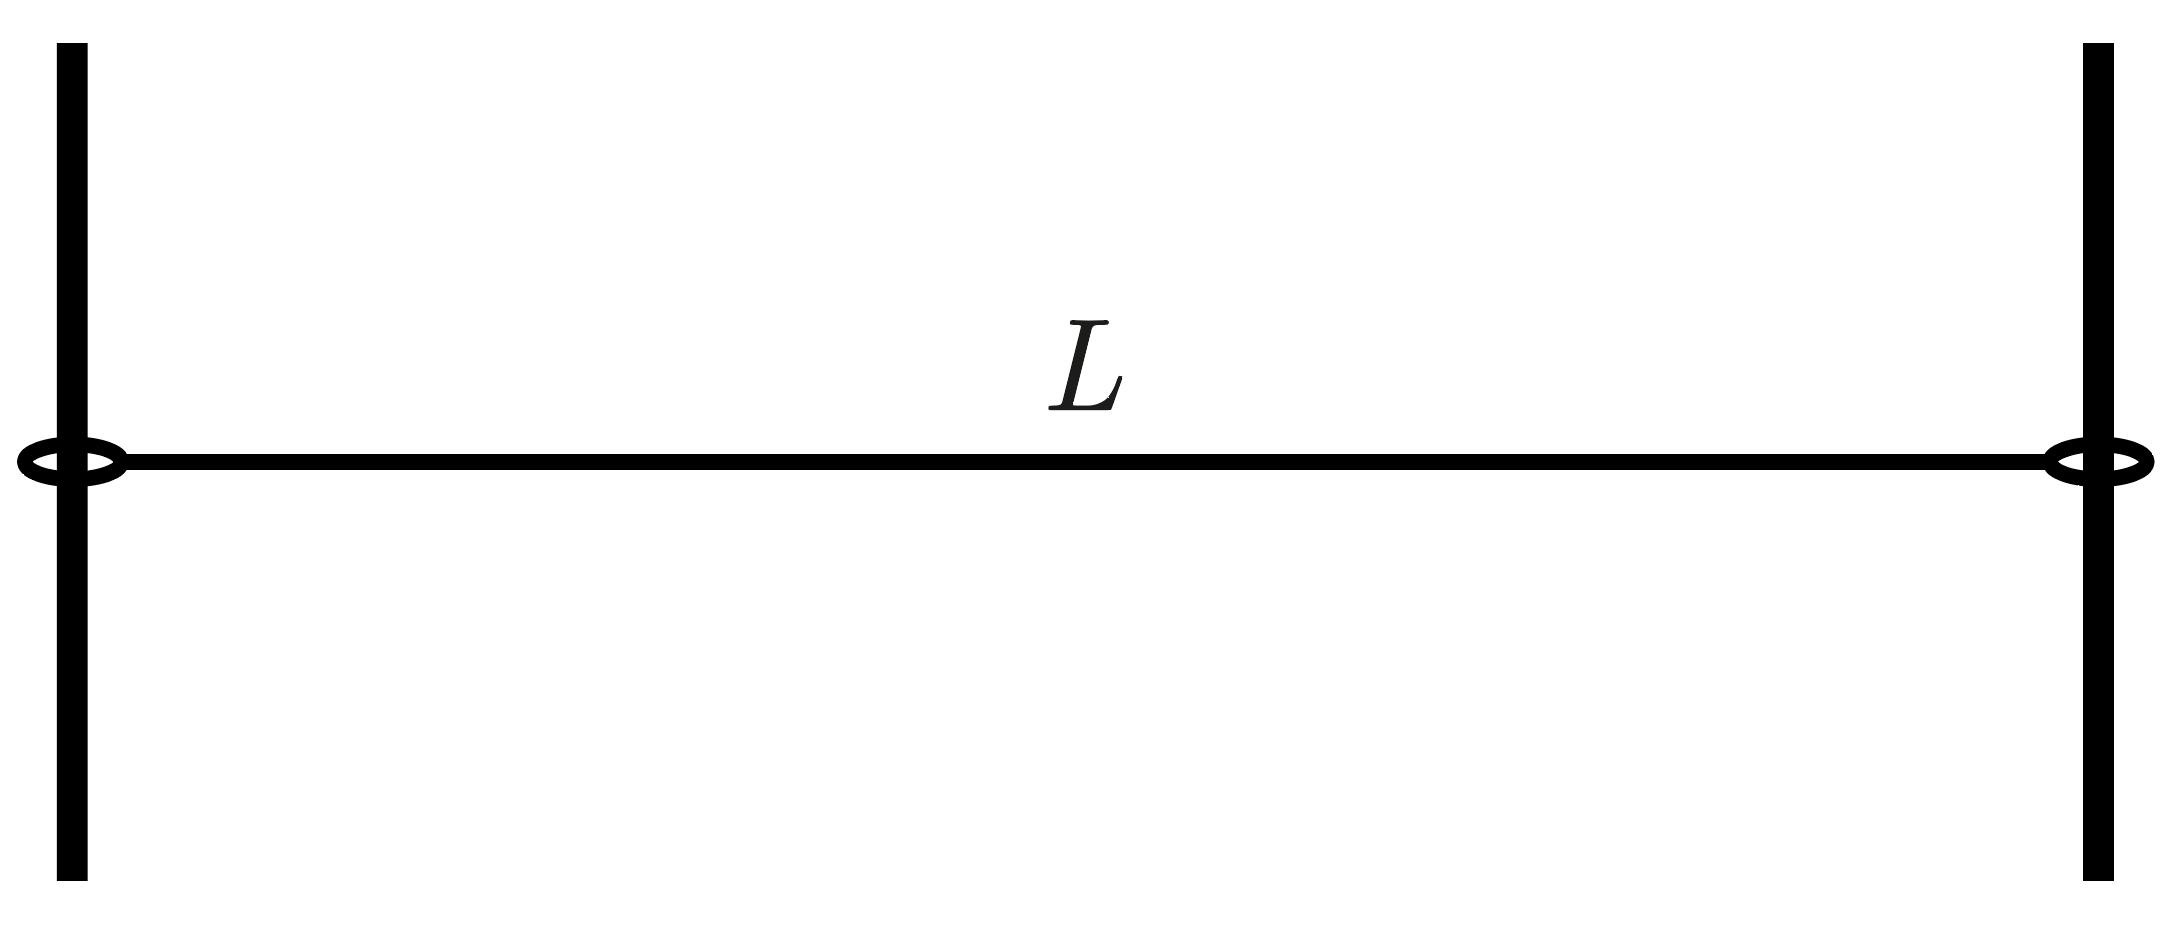
\includegraphics[width=7.5cm]{loose-ends.png}
    \end{center}
\end{prob}
\begin{sol}
    We must have that the slope at the ends is equal to $0$,
    $$\frac{\partial}{\partial x}\psi(0,t) = 0, \frac{\partial}{\partial x}\psi(L,t) = 0.$$
    So, we need
    $$kL = n\pi \implies k = \frac{n\pi}{L}.$$
    So, the frequency of normal modes are $\omega = ck = \frac{cn\pi}{L}$. The actual normal modes are gonna be standing waves with
    $$f(x) = \cos(kx) = \cos(n\pi x/L).$$
\end{sol}

%standing waves / boundary condition problems

%wave energy problem + power transmission

\begin{prob}
    Consider a string of mass density $\rho$ and tension $T$. A wave pulse given by $\psi(x,t)$ travels through it.
    \begin{anum}
        \item Compute the kinetic and potential energy density of the string as a function of $x$ and $t$. 
        \item Compute the densities for the standard traveling sinusoidal wave $A \cos (kx - \omega t)$ and a general traveling wave $\psi = f(x-vt)$.
        \item Find an expression for the power flowing across the point $x = x_0$ as a function of time for the wave $\psi = A \cos (kx - \omega t)$.
    \end{anum}
\end{prob}
\begin{alphasol}
    \item The kinetic energy of a given point is given by its speed, $\dot \psi^2$. So, the KE density is
    $$KE = \frac 12 \rho \dot \psi ^2 (x,t).$$
    Now, for the potential energy density, we need to look at how much the string between $x$ and $x+dx$ is stretched. Using the pythagorean theorem,
    $$PE \, dx = T\left(\sqrt{dx^2 + \left(\frac{\partial \psi}{\partial x}dx\right)^2} - dx\right) = (Tdx) \left(1 + \frac 12 \left(\frac{\partial \psi}{\partial x}\right)^2 - 1\right) = \frac 12 T \psi'^2(x,t)\, dx,$$
    giving us the PE density.
    \item For the general case, we have
    $$KE = \frac 12 \rho v^2 f(x-vt)^2, PE = \frac 12 T f(x-vt)^2.$$
    And for a string wave, $v^2 = T/\rho$, so we see that the KE and PE densities are the same. For the cosine wave, $f(x) = A\cos(kx)$, so
    $$KE = \frac 12 \rho v^2 A^2 \cos^2(kx - \omega t), PE = \frac 12 T A^2 \cos^2(kx - \omega t).$$
\end{alphasol}


%sketching waves????

\begin{prob}
    Using ideas from problem \ref{pr:essential}, sketch the time evolution of the following transverse string waves with drawn initial positions which are released from rest. Make sure to include a picture before and after the wave pulses reflect off of the walls. Let $v$ be the wave speed of the string.
    \begin{anum}%include hard and soft wall reflections
        \item Draw the general progression along with specific plots at times $t= \frac{L}{4v}$ and $t = \frac{L}{v}$.
        \begin{center}
            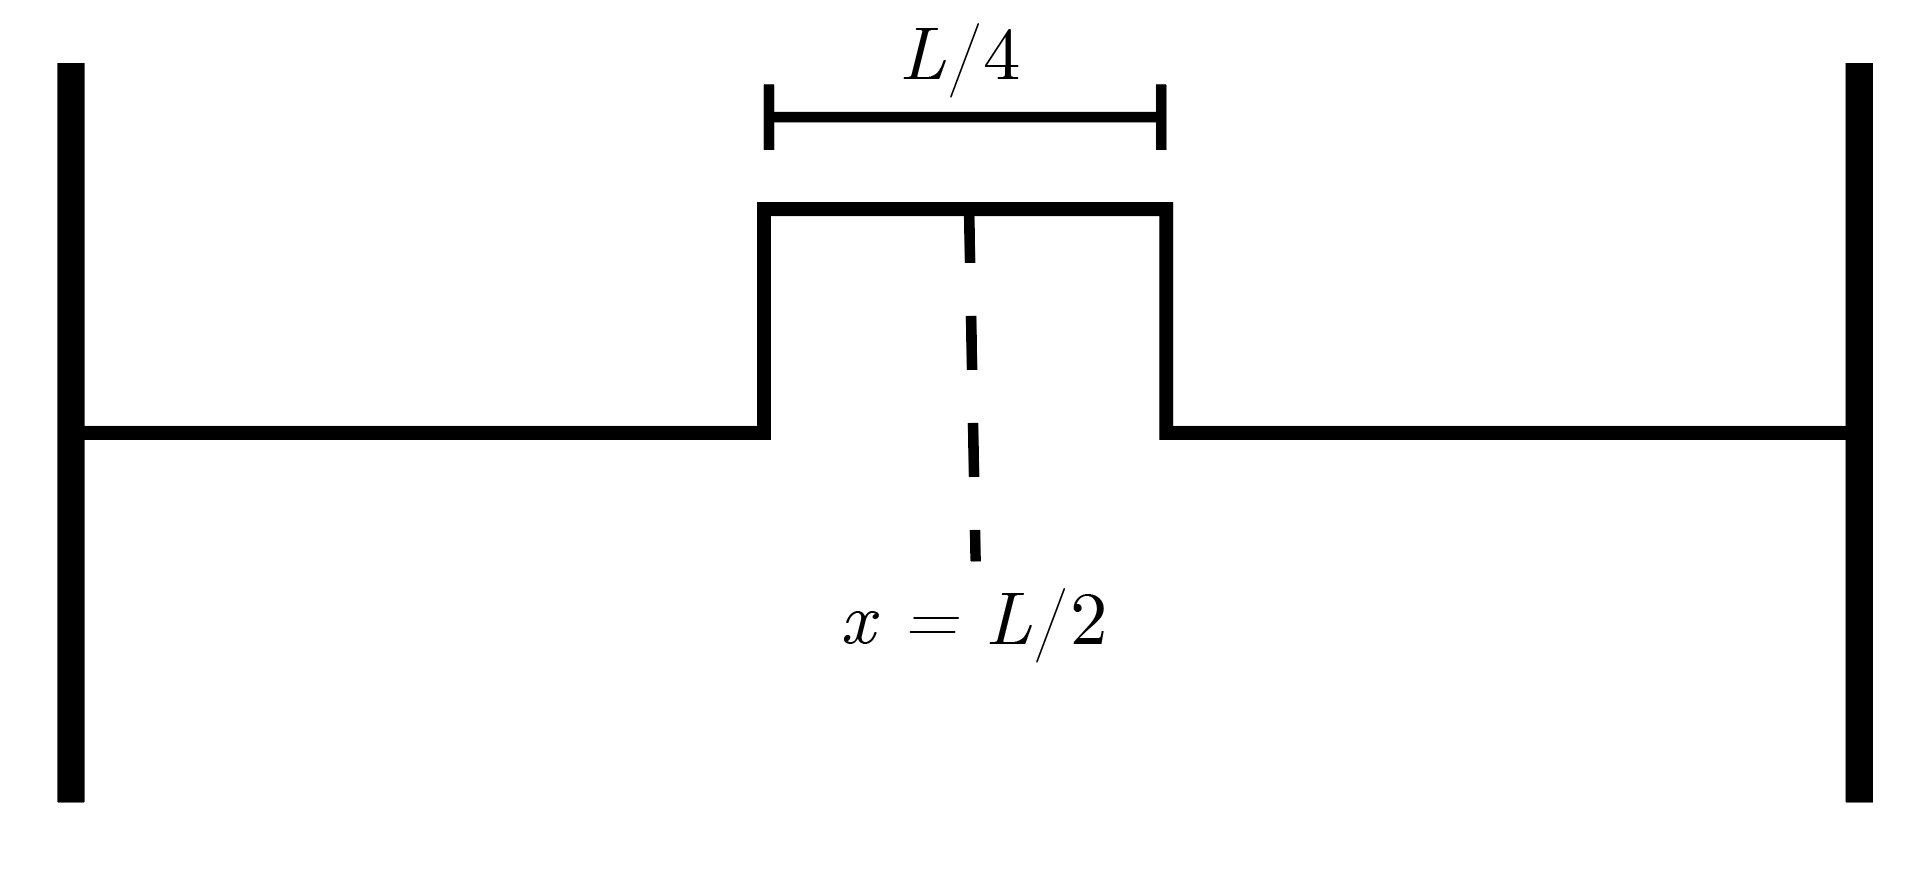
\includegraphics[width=7.5cm]{wave_1.png}
        \end{center}
        \item Draw the general progression along with specific plots at times $t= \frac{L}{4v}$ and $t = \frac{L}{v}$.
        \begin{center}
            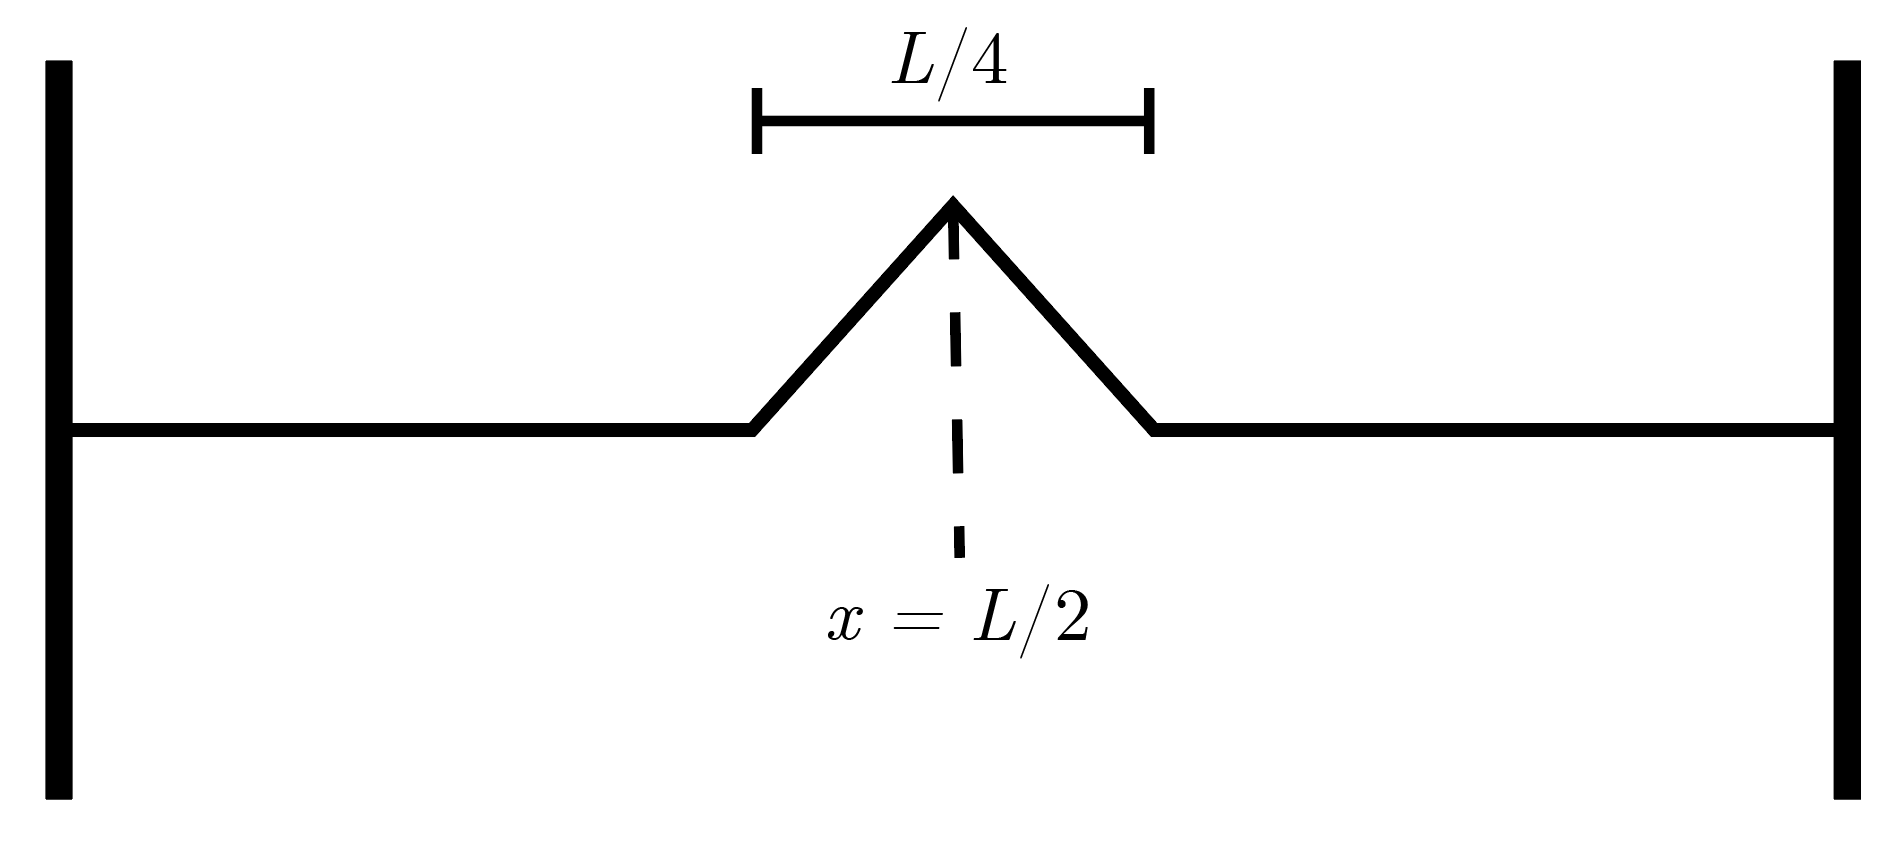
\includegraphics[width=7.5cm]{wave_2.png}
        \end{center}
    \end{anum}
\end{prob}
\begin{sol}
    The idea here is that these are composed of two waveforms of half the height moving in opposite directions at speed $v$. So, at time $t = L/4v$, both of the two would've shifted by a distance $L/4$. Meanwhile, at time $L/v$, the waves travel a distance $L$, which means hitting the walls and coming back to the center, but with a $\pi$ shift. Thus, the second case leads to just a flipped version of the wave for both (a) and (b). The plots are drawn below.
    \begin{center}
        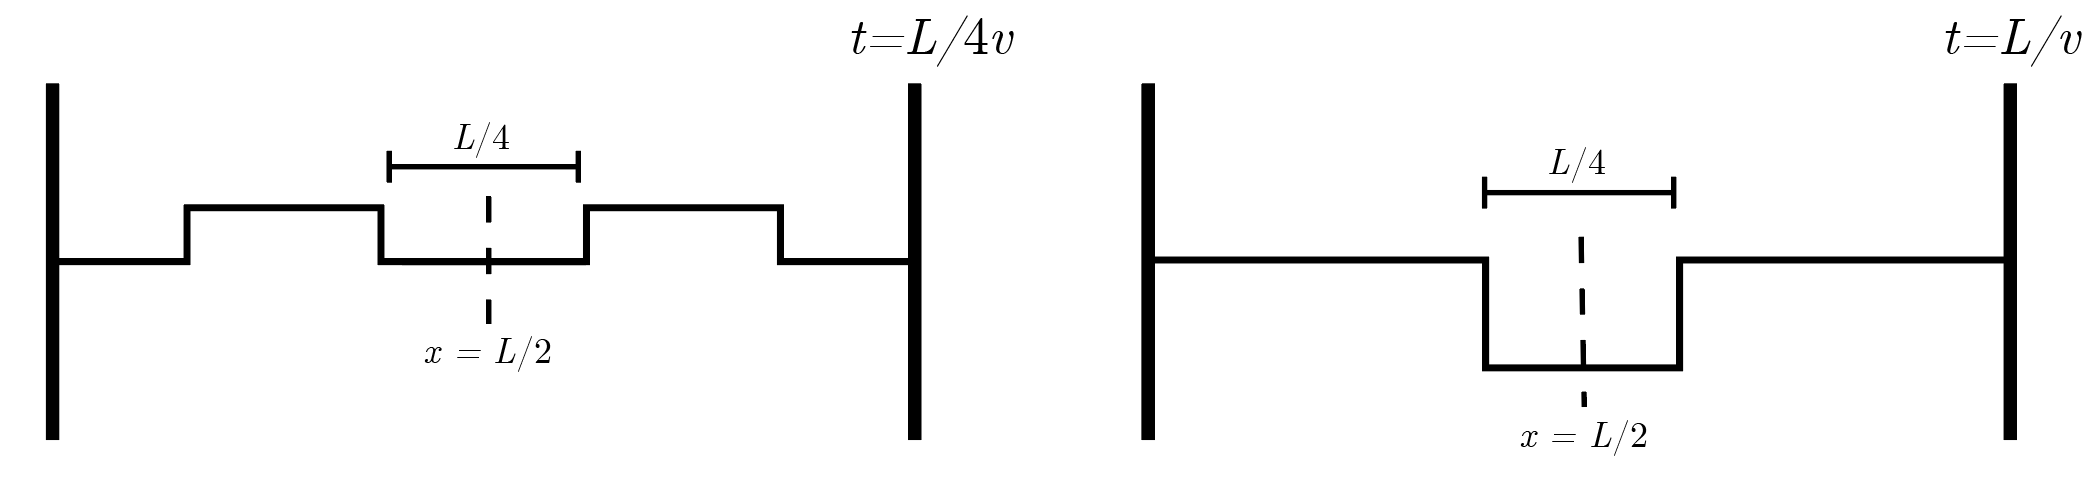
\includegraphics[width=13cm]{rect-sol.png}
        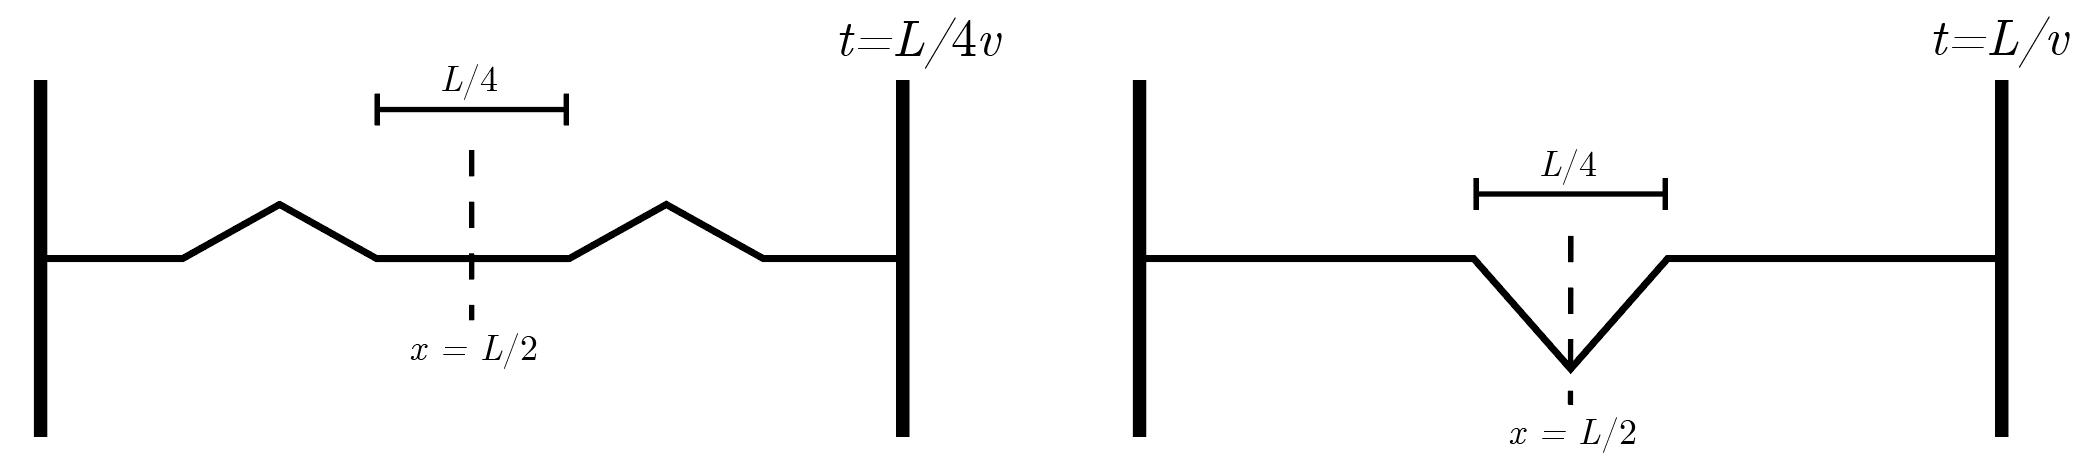
\includegraphics[width=13cm]{triangle-sol.png}
    \end{center}
\end{sol}


%reflection transmission????
\begin{prob}[MIT]
    Consider two strings with mass density $\mu_1 = \mu$ and $\mu_2 = \mu / 2$ and tensions $T_1 = T$ and $T_2 = T /2$
connected by a massless ring at $x = 0$. The ring can move along a frictionless rod. String 1 extends to the left, far beyond $x = -L$, and string 2 is attached to a fixed point on the wall at $x = L$. Initially a triangular pulse of width $L/4$ is moving along string 1 from left to right. At $t=0$ the front
edge of the triangle is at $x = -7L/8$ as shown below.
\begin{center}
    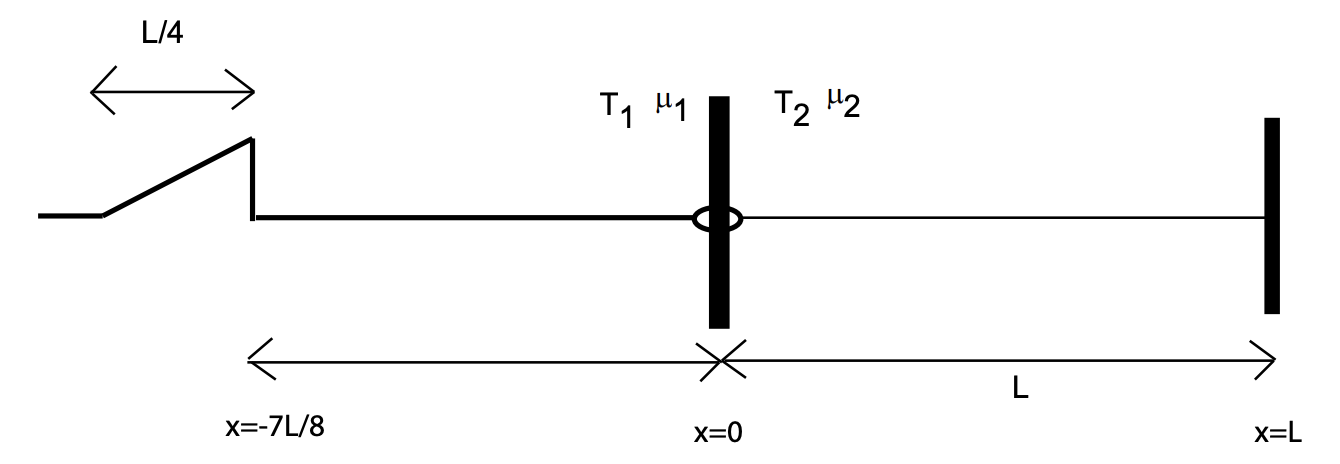
\includegraphics[width=7.5cm]{traveling_triangle.png}
\end{center}
\begin{anum}
    \item Write wave equations on both sides of the ring and specify the boundary conditions at $x=0$.
    \item Do you expect reflected waves at $x = 0$ and at $x = L$? Will the reflected wave have the same or the opposite sign than the incoming wave at $x = 0$ and at $x = L$?
    \item Assume that the incoming pulse is of the form $f_1(x,t) = f_1(x/v_1 - t)$. Find the functional form of the transmitted $g(x,t)$ and reflected $f_2(x,t)$ pulses at $x = 0$ and $x = L$. Consider only times $t \le 2L \sqrt{\frac \mu T}$.
    \item Make a sketch of string deformations at $t = L \sqrt{\frac \mu T}$ and $t = 2L\sqrt{\frac\mu T}$.
\end{anum}
\end{prob}
\begin{alphasol}
    \item The wave equation on both sides is the same as $\sqrt{T/\mu}$ is the same on both sides,
    $$\frac{\partial^2 y}{\partial x^2} = \frac{\mu}{T}\frac{\partial^2 y}{\partial t^2}.$$
    The boundary condition is no force on the ring, so
    $$T\left.\frac{\partial y}{\partial x}\right|_{x=0^-} = \frac T2 \left. \frac{\partial y}{\partial x}\right|_{x=0^+}.$$
    \item The right wall is a normal hard wall, so we expect a reflection, and one of opposite sign. For the center point, the right side has lower impedance, so we expect that it reflects with the same phase.
    \item We write down the boundary condition using these waves,
    $$\frac{1}{v_1}f_1(x/v_1 - t) -\frac{1}{v_1}g(-x/v_1 - t) = \frac 12 \frac{1}{v_2}f_2(x/v_2 - t).$$
    Cancelling $v_1 = v_2$ and plugging in $x= 0$, we get
    $$f_1(-t) - g(-t) = \frac 12 f_2(-t).$$
    Further, by continuity,
    $$f_1(-t) + g(-t) = f_2(-t),$$
    so $$2f_1(-t) = \frac 32 f_2(-t) \implies f_2(t) = \frac 43 f_1(t).$$
    Putting that back in, we get $g(-t) = \frac 13 f_1(-t)$, so
    $$g(x,t) = \frac 13 f_1(-x/v_1 - t), f_2(x,t) = \frac 43 f_1(x/v_1 - t).$$
    At $x=L$ it is simple as the point is fixed, so $$f_2 = 0, g(x,t) = - f_1(-x/v_1 - t).$$
    \item The first time point is when it has travelled a distance $L$, so that the pulse is halfway into the pole. The second time is when the reflected has returned fully and when the transmitted has passed the wall. The green corresponds to $t = 2L\sqrt{\mu/T}$ and the blue corresponds to $t= L\sqrt{\mu/T}$.
    \begin{center}
        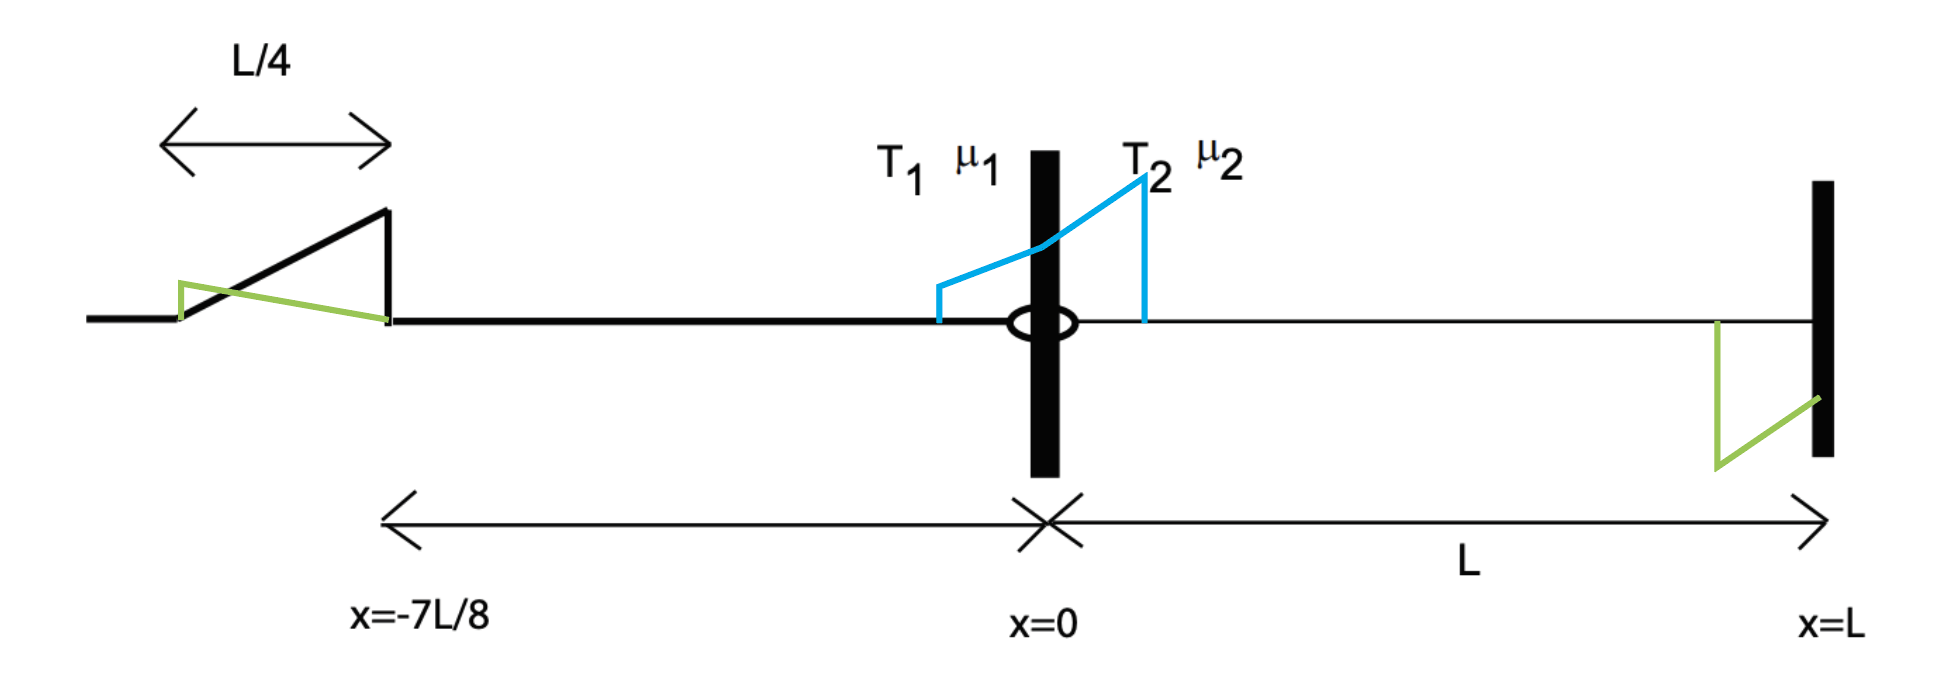
\includegraphics[width=7.5cm]{waves_travel.png}
    \end{center}
\end{alphasol}

%refraction

\begin{prob}
    \href{https://www.aapt.org/physicsteam/upload/2022-USAPhO-Exam.pdf#page=6}{USAPhO 2022/A3}, a problem that explains an everyday physical phenomenon!
\end{prob}
\begin{sol}
    \officialsol{https://aapt.org/physicsteam/upload/2022-USAPhO-solutions.pdf}
\end{sol}

\begin{prob}
    Optical fibers are used to transmit information much faster than standard electric cables. They operate on the basis of total internal reflection, consisting of a core of index of refraction $n_1$ and a cladding of index of refraction $n_2 < n_1$. What is the maximum angle $\theta$ that light can be incident on the setup below such that the beam is contained within the core for the entire length?
    \begin{center}
        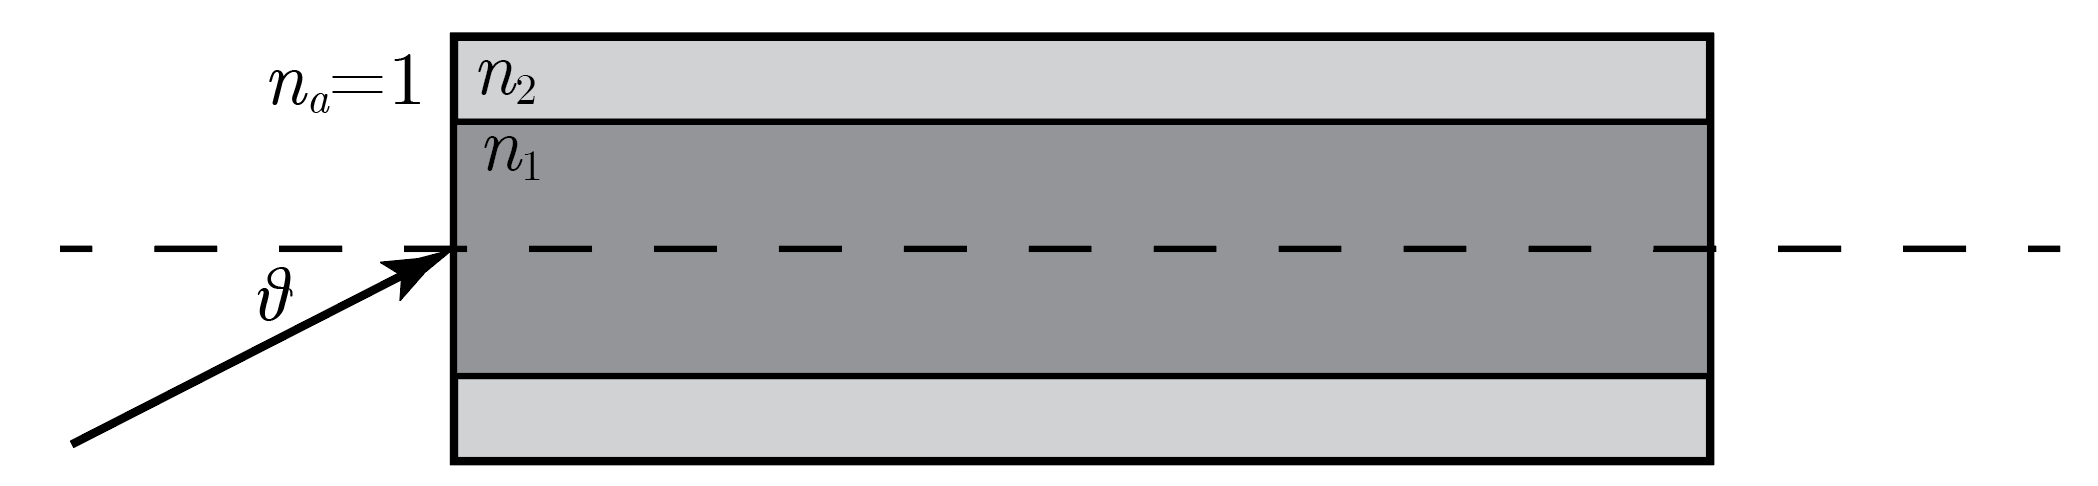
\includegraphics[width=10cm]{optic_fiber.png}
    \end{center}
\end{prob}
\begin{sol}
    Suppose the ray enters the core with an angle of incidence $\phi$. Then, we find the critical angle at the core and cladding boundary,
    $$n_1 \sin(90 - \phi) = n_2 \sin(90^\circ) = n_2 \implies \phi = \cos^{-1}(n_2/n_1).$$
    Now, we apply snell's law on the other boundary,
    $$\sin \theta = n_1 \sin (\phi) = n_1 \frac{\sqrt{n_1^2 - n_2^2}}{n_1} = \sqrt{n_1^2 - n_2^2},$$
    giving $\theta = \boxed{\sin^{-1}\left(\sqrt{n_1^2 - n_2^2}\right)}$.
\end{sol}

\begin{prob}
    \href{https://ipho.olimpicos.net/pdf/IPhO_1984_Q1.pdf}{IPhO 1984/T1}, another physical phenomenon!
\end{prob}
\begin{sol}
    \officialsol{https://ipho.olimpicos.net/pdf/IPhO_1984_S4.pdf}
\end{sol}
%doppler
\begin{prob}
    \href{https://olympiads.hbcse.tifr.res.in/wp-content/uploads/2020/02/INPHO2020-Questions-en.pdf}{INPhO 2020/4}, a tricky graphical doppler effect problem.
\end{prob}
\begin{sol}
    \officialsol{https://olympiads.hbcse.tifr.res.in/wp-content/uploads/2020/03/INPHO2020-Solutions-20200220.pdf}
\end{sol}
\begin{prob}
    \href{https://www.aapt.org/physicsteam/2016/upload/E3-2-3.pdf}{USAPhO 2016/A1}, another tricky graphical doppler effect problem.
\end{prob}
\begin{sol}
    \officialsol{https://aapt.org/physicsteam/upload/USAPhO-2016-Solutions.pdf}
\end{sol}

\begin{prob}[Wang]
    A car travels at speed $v$ in the lab frame along horizontal ground and emits
waves of speed $u$ in the lab frame at frequency $f$. If the car is receding from
a stationary vertical wall (in a direction normal to the wall), determine the
frequency of the reflected waves that are received by the car.
\end{prob}
\begin{sol}
    First, the frequency of the waves is redshifted in the lab frame,
    $$f' = \frac{u}{u + v}f.$$
    Then, after this reflects, the car becomes the observer, and there is a second doppler effect, leading to
    $$f'' = \frac{u-v}{u}\frac{u}{u+v}f = \frac{u-v}{u+v}f.$$
\end{sol}


\subsection{Challenge Problems}

\begin{prob}
    \href{https://eupho.ee/wp-content/uploads/2020/07/EuPhO17_theory.pdf}{EuPhO 2017/T1}
\end{prob}
\begin{sol}
    \officialsol{https://eupho.ee/wp-content/uploads/2020/07/EuPhO17_theory_solution_marking.pdf}
\end{sol}

\subsection{USAPhO Practice}

\begin{prob}[USAPhO 2008/A4]
    A tape recorder playing a single tone of frequency $f_0$ is dropped from rest at a height $h$. You stand directly
underneath the tape recorder and measure the frequency observed as a function of time. Here $t = 0$ s is the time at which the tape recorder was dropped.
\begin{center}
    \begin{tabular}{c|c}
        $t$ (s) & $f$ (Hz) \\ \hline
        2.0 & 581\\
        4.0 & 619\\
        6.0 & 665\\
        8.0 & 723\\
        10.0 & 801
    \end{tabular}
\end{center}
The acceleration due to gravity is $g=9.80\,\unit{m/s^2}$ and the speed of sound in air is $v_{\text{snd}} = 340\,\unit{m/s}$. Ignore air resistance. You might need to use the Doppler shift formula for co-linear motion of sources and observers in still air,
$$f = f_0 \frac{v_{\text{snd}} \pm v_{\text{obs}}}{v_{\text{snd}} \pm v_{\text{src}}}.$$
where $f_0$ is the emitted frequency as determined by the source, $f$ is the frequency as detected by the observer,
and $v_{\text{snd}}$, $v_{\text{src}}$, and $v_{\text{obs}}$ are the speed of sound in air, the speed of the source, and the speed of the observer. The positive and negative signs are dependent upon the relative directions of the motions of the source and the observer.
\begin{anum}
    \item Determine the frequency measured on the ground at time $t$, in terms of $f_0$, $g$, $h$, and $v_{\text{snd}}$. Consider only the case where the falling tape recorder doesn’t exceed the speed of sound $v_{\text{snd}}$.
    \item Verify graphically that your result is consistent with the provided data.
    \item What (numerically) is the frequency played by the tape recorder?
    \item From what height $h$ was the tape recorder dropped?
\end{anum}
\end{prob}
\begin{sol}
    \officialsol{https://aapt.org/Common/upload/USAPhO-2008-Solutions_rev-4012021.pdf}
\end{sol}

\begin{prob}
    Consider a tube filled with air of average density $\rho_0$ and adiabatic factor $\gamma$, cross-sectional area $A$, and average pressure $P_0$. In this problem, we calculate the speed of sound within this tube. Let $\rho(x), v(x), P(x)$ be the density, velocity, and pressure distributions across the tube. Assume that all processes are adiabatic, $v^2 \ll P/\rho$, and all fluctuations in $\rho,v,P$ are much smaller than their average magnitude.
    \begin{anum}
        \item Write down a differential equation relating $\rho(x)$ and $P(x)$.
        \item Consider a parcel of air between $x$ and $x+dx$. Now, write down a differential equation involving $v$ and $\rho$ only, using Newton's second law. \textit{Hint:} some of the derivatives may be with respect to time, and others may be with respect to position.
        \item Write down a second differential equation involving $v$ and $\rho$ only by using continuity.
        \item Finish by reducing your differential equations to a wave equation in one of the variables,
        $$\frac{\partial^2 (?)}{\partial x^2} = \frac 1{c^2} \frac{\partial^2 (?)}{\partial t^2}.$$
        and read off the speed of sound $c$. Is $c^2 \ll P/\rho$? If not, are our assumptions at the start of the problem valid?
        \item At the start of the problem we made the assumption that $v \ll P/ \rho$. Where does the derivation breakdown if this was not true?
    \end{anum}
\end{prob}
\begin{alphasol}
    \item Because the processes are adiabatic, we can write down the adiabatic invariant. We have $V \propto \frac{1}{\rho}$, so
    $$PV^\gamma \propto P\rho^{-\gamma} = \text{const.}$$
    Thus, differentiating, we get
    $$\frac{dP}{P} - \gamma \frac{d\rho}{\rho} = 0.$$
    \item We consider the pressure on both sides,
    $$F = A\Delta P = A\frac{\partial P}{\partial x} dx.$$
    We can equate this to
    $$ma = \rho A dx \frac{\partial v}{\partial t} = A \frac{\partial P}{\partial x} dx.$$
    So, our differential eqn is
    $$\rho \frac{\partial v}{\partial t} = \frac{\partial P}{\partial x}.$$
    \item We must have that the change in density within a given region is equal to the amount of ``stuff'' that flows in. The amount of stuff that flows in can be calculated from the difference in velocities from the left and right sides of the box. So,
    $$A dx \frac{\partial \rho}{\partial t} = \rho A \frac{\partial v}{\partial x} dx \implies \pdv{\rho}{t} = \rho \pdv{v}{x}.$$
    \item We can write 
    \begin{align*}
        \pdv[2]{\rho}{t} &= \rho \pdv{v}{t}{x},\\
        &= \pdv{x}\pdv{P}{x},\\
        &= \frac{\gamma P}{\rho} \pdv[2]{\rho}{x}.
    \end{align*}
    Thus, we get that $c= \sqrt{\gamma P/\rho}$. It is on the order $\sqrt{P/\rho}$, but this is not a problem because the speed of the wave is different from the speed of the particles in the wave.
    \item The $F=ma$ equation breaks down. We assume that we're essentially working with the same set of mass when we take the partial derivative with respect to $v$. However, with a sufficiently fast speed, the set of particles that you're calculating the force on changes in the time $dt$, and you have to account for that change. Furthermore, if it gets fast enough and break the sound barrier, pressure and density are not even well-defined due to shock waves.
\end{alphasol}


\end{document}